\documentclass[3pt,landscape]{article}
%ss[10pt,landscape]{article}
\usepackage{multicol}
\usepackage{calc}
\usepackage{ifthen}
\usepackage[landscape]{geometry}
\usepackage{amsmath,amsthm,amsfonts,amssymb}
\usepackage{color,graphicx,overpic}
\usepackage{hyperref}


\pdfinfo{
/Title (final.pdf)
/Creator (TeX)
/Producer (pdfTeX 1.40.0)
/Author (Raemond Bergstrom-Wood)
/Subject (Networks)
/Keywords (pdflatex, latex,pdftex,tex)}

% This sets page margins to .5 inch if using letter paper, and to 1cm
% if using A4 paper. (This probably isn't strictly necessary.)
% If using another size paper, use default 1cm margins.
\ifthenelse{\lengthtest { \paperwidth = 11in}}
    { \geometry{top=.3in,left=.3in,right=.3in,bottom=.3in} }
    {\ifthenelse{ \lengthtest{ \paperwidth = 297mm}}
        {\geometry{top=1cm,left=1cm,right=1cm,bottom=1cm} }
        {\geometry{top=1cm,left=1cm,right=1cm,bottom=1cm} }
    }

% Turn off header and footer
\pagestyle{empty}

% Redefine section commands to use less space
\makeatletter
\renewcommand{\section}{\@startsection{section}{1}{0mm}%
                            {-1ex plus -.5ex minus -.2ex}%
                            {0.5ex plus .2ex}%x
                            {\normalfont\large\bfseries}}
\renewcommand{\subsection}{\@startsection{subsection}{2}{0mm}%
                            {-1explus -.5ex minus -.2ex}%
                            {0.5ex plus .2ex}%
                            {\normalfont\normalsize\bfseries}}
\renewcommand{\subsubsection}{\@startsection{subsubsection}{3}{0mm}%
                            {-1ex plus -.5ex minus -.2ex}%
                            {1ex plus .2ex}%
                            {\normalfont\small\bfseries}}
\makeatother

% Define BibTeX command
\def\BibTeX{{\rm B\kern-.05em{\sc i\kern-.025em b}\kern-.08em
    T\kern-.1667em\lower.7ex\hbox{E}\kern-.125emX}}

% Don't print section numbers
\setcounter{secnumdepth}{0}


\setlength{\parindent}{0pt}
\setlength{\parskip}{0pt plus 0.5ex}

%My Environments
\newtheorem{example}[section]{Example}
% -----------------------------------------------------------------------

\def\ci{\perp\!\!\!\perp}

\begin{document}
\raggedright
\footnotesize
\begin{multicols}{3}


% multicol parameters
% These lengths are set only within the two main columns
%\setlength{\columnseprule}{0.25pt}
\setlength{\premulticols}{1pt}
\setlength{\postmulticols}{1pt}
\setlength{\multicolsep}{1pt}
\setlength{\columnsep}{2pt}

\begin{center}
    \Large{\underline{EE 122 Final Note Sheet}} \\
\end{center}

\subsection*{Domain Name System (DNS)}
\subsubsection*{Internet Names \& Addresses}
\begin{itemize}
    \item Machine Addresses: e.g., 169.229.131.101
        \begin{itemize}
            \item reouter-usable labels for machines
            \item conforms to network structure (the "where")
        \end{itemize}
    \item Machine Names: e.g., instr.eecs.berkeley.edu
        \begin{itemize}
            \item human-usable labels for machines
            \item conforms to organizational structure ("the who")
        \end{itemize}
    \item The Domain Name System (DNS) is how we map from one to the other.
\end{itemize}

\subsubsection*{Goals of DNS}
\begin{itemize}
    \item No naming conflicts (uniqueness)
    \item Scalable (many names and frequent updates)
    \item Distributed, autonomous administration
        \begin{itemize}
            \item Ability to update my own machines names
            \item Don't have to track all updates
        \end{itemize}
    \item Highly available
    \item Lookups are fast
\end{itemize}

\subsubsection*{DNS Hierarchy}
Made up of three intertwined hierarchies
\begin{itemize}
    \item Hierarchical namespace, as opposed to the original flat namespace.
    \item Hierarchically administered, as opposed to centralized
    \item (Distributed) Hierarchy of servers, as opposed to centralized storage.
\end{itemize}

\subsubsection*{Domain Resolution}
\begin{center}
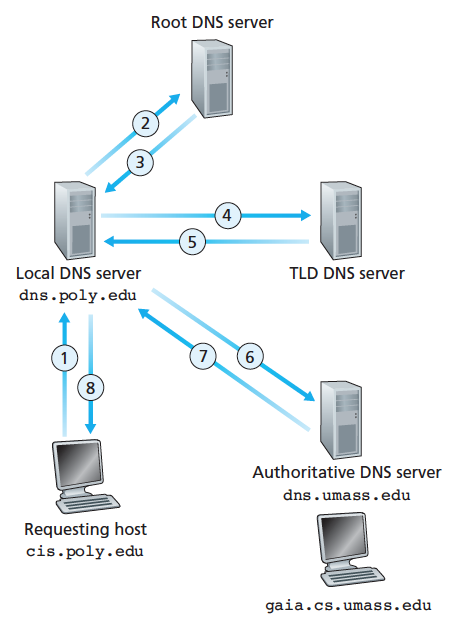
\includegraphics[scale=.2]{DNSResolution}
\end{center}
\begin{itemize}
    \item Recursive query, asks the server to get you the answer.
    \item Iterative quere, asks the server to give you the next server to check.
\end{itemize}

\subsubsection*{DNS Records}
DNS info is stored as resource records (RRs)
\begin{itemize}
    \item Address: name = hostname, value = IP Address
    \item Name Server: name = domain, value = name of dns server for domain
    \item Canonical NAME: name = hostname, value = canonical name
    \item Mail eXchanger: name = domain in email address, value = canonical name of mail server
\end{itemize}

\subsubsection*{DNS Protocol}
Client-Server interaction is on UDP Port 53

\subsubsection*{DNS Caching}
\begin{itemize}
    \item DNS servers cache responses to queries
    \item Responses include a TTL field and the server deletes the cached entry after the TTL expires
    \item Negative Caching: misspellings like cnn.comm take a long time to fail the first time. Some servers implement a cache of mistakes, but it is optional and not widely implemented.
\end{itemize}

\subsection*{Hyper Text Transfer Protocol (HTTP)}
\subsubsection*{Uniform Record Locator (URL)}
Web content is named using URLs, URLs use DNS hostnames

\subsubsection*{HTTProtocol}
\begin{itemize}
    \item Stateless
        \begin{itemize}
            \item Each request-response is treated independently, servers do not retain state
            \item Good: This improves server-side scalability, failure handling
            \item Bad: Some application need persistent state (ex, shopping carts, user profiles, ect.)
        \end{itemize}
    \item HTTP runs over TCP on port 80
    \item Synchronous request/reply protocol
\end{itemize}

\subsubsection*{Steps in an HTTP Request/Response}
\begin{center}
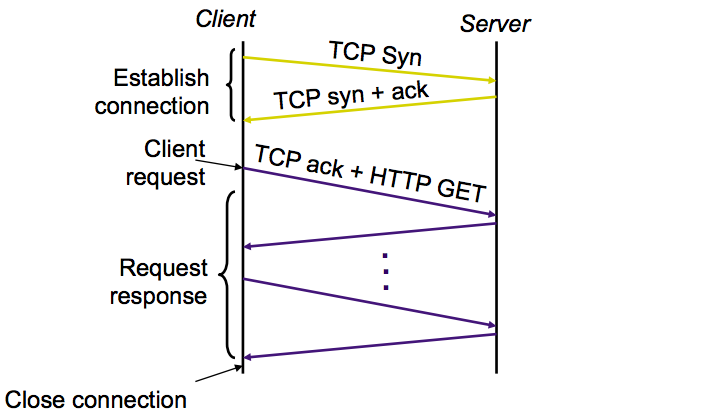
\includegraphics[scale=.3]{HTTPRequestResponse}
\end{center}

\subsubsection*{Client-to-Server Communication}
\begin{itemize}
    \item HTTP Request Message
        \begin{itemize}
            \item Request line: method, resource, and protocol version
            \item Request headers: provid information or modify request
            \item Body: optional data (ex, "POST" data to the server)
        \end{itemize}
    \item HTTP Response Message
        \begin{itemize}
            \item Status line: Protocol version, status code, status phrase
            \item Response headers: provide information
            \item Body: optional data
        \end{itemize}
\end{itemize}

\subsubsection*{HTTP Performance}
Most web pages have multiple objects. Naively, this would be one tcp connection per (possibly small) object.
\begin{itemize}
    \item Concurrent Requests and Responses
        \begin{itemize}
            \item Uses multiple connects in parallel
            \item Doesn't necessarily maintain the order of responses.
        \end{itemize}
    \item Persistent Connections
        \begin{itemize}
            \item Maintain TCP connection across multiple requests. (including transfers from the current page.) Either the cliet or the server can tear down the connection.
            \item This avoids overhead of connection set-up and tear-down, creates a more accurate RTT estimate, allows TCP congestion window to increase. (Thereby being able to use previosly discovered bandwidth.)
            \item default in HTTP/1.1
        \end{itemize}
    \item Pipelined Requests
        \begin{itemize}
            \item Batch requests and responses to reduce the number of packets
            \item Multiple requests can be contained in one TCP segment
        \end{itemize}
    \item Getting n Large Objects
\end{itemize}
\begin{tabular}{|l|c|c|}
    \hline
    Connection Style & latency & bandwidth\\
    \hline
    \hline
    One-at-a-time & ~2n RTT & ~nF/B\\
    M concurrent & ~[n/m] RTT & ~[n/m] F/B\\
    Persistent & ~(n+1) RTT & ~nF/B\\
    Pipelined & ~2 RTT & ~nF/B\\
    Pipelined/Persistent & ~2 RTT then RTT later & ~nF/B\\
    \hline
\end{tabular}
\begin{itemize}
    \item Caching
        \begin{itemize}
            \item Adds the modifier, "If-modified-since", os if the resource hasn't changed, it simply returns "not modified"
            \item The response header has field, "Expires" that tells it how long it is safe to cache and "No-cache" which will ignore caches and always get the resource.
            \item Client Caching: on your computer.
            \item Forward Proxies: Done by ISPs to reduce network traffic and lower latency
            \item Reverse Proxies: Done close to the server to reduce server load. Usually done by the content provider.
        \end{itemize}
    \item Replication
        \begin{itemize}
            \item Replicates popular web sites across multiple machines. This spreads load on servers, places content closer to clients, and helps when content isn't cacheable. To account for locationality, DNS returns different addresses based on client's geo location, server load, ect.
        \end{itemize}
\end{itemize}
% You can even have references
\rule{0.3\linewidth}{0.25pt}
\scriptsize
\bibliographystyle{abstract}
\bibliography{refFile}
\end{multicols}
\end{document}
